\section{INTRODUCTION}\label{sec:1introduction}

Sleep plays a vital role in good health and personal well-being throughout one's life. Lack of sleep or poor quality of sleep can lead to
serious, sometimes life-threatening, health problems~\cite{altena2008sleep,chandola2010effect,lallukka2016contribution}, decrease level of
cognitive performance~\cite{alhola07sleep,akerstedt07altered}, and affect mood and feelings of personal
well-being~\cite{paunio09longitudinal,pilcher97sleep}. Besides having an adverse effect on individuals, insufficient or poor quality sleep
has a significant economic burden, among others, through decreased productivity, and medical and social costs associated with treatment of
sleep disorders~\cite{hafner17why}. Indeed, to highlight the significance of sleep quality, the Centre for Disease Prevention (CDC) has
declared insufficient sleep as a public health problem in the US~\cite{sleepreport}, and the concern is widely shared amongst other
industrialized countries.

Traditionally, sleep monitoring is performed in a clinical environment using Polysomnography (PSG). In PSG, medical sensors attached to
human body are used to monitor events and information such as respiration, electroencephalogram (EEG), electrocardiogram (ECG),
electro-oculogram and oxygen saturation~\cite{ebrahimi2008automatic,saper2005hypothalamic,oropesa1999sleep,langkvist2012sleep}. These
information sources can then be used to determine
sleep stages, sleep efficiency, abnormal breathing, and overall sleep quality. While PSG is widely considered as the gold standard for sleep monitoring, and while it is extensively used to support clinical treatments of sleep disorders, it has some disadvantages that make it unsuitable for longitudinal and large-scale sleep monitoring. Firstly, the sensing instruments are time-consuming and laborious to put on, and they are prone to disrupting sleeping routines.  Secondly, PSG is rather expensive to use and requires a clinical environment and highly trained medical professionals to operate. Due to these disadvantages, PSG is only suitable as a way to support severe disorders that clinical care is required. %These disadvantages restrict PSG to be used as a day to day sleep monitoring method.


Recently, sleep monitoring based on off-the-shelf mobile and wearable devices has emerged as an alternative way to obtain information about
one's sleeping patterns~\cite{ko15consumer,shelgikar2016sleep}. By taking advantage of diverse sensors, behaviours and routines associated
with sleeping can be captured and modelled. This in turn can help users understand their sleep behaviour and provide feedback on how to
improve their sleep, for example, by changing routines surrounding sleep activity or improving the sleeping environment. What makes self
monitoring particularly attractive is the non-invasive nature of the sensing compared to PSG. Examples of consumer-grade sleep monitors
range from apps running on smartphones or tablets to smartwatches and specialized wearable
devices~\cite{zeo,Jawbone,SleepAndroid,fitbit,gu2016sleep,sleepmonitor}.

%Sleep monitoring using consumer-grade devices is also known as \emph{actigraphy}~\cite{Actigraphy,ancoli2003role} as the key goal is to capture and characterize periods of inadct
%Traditionally, sleep monitoring had to be performed in a clinic environment using dedicated medical equipment.  Modern mobile devices such
%as smartphones and wearable devices offer a new way for sleep monitoring. By utilizing the rich mobile sensors, we can track certain
%activities such as body movements or snore, and to use the tracked information to detect and model sleep
%patterns. Such an approach is known as
%. Compared to a clinic solution, an actigraphy approach the advantages of being lower
%cost and non-invasive, and can be performed at home on an on-going basis.

%Current solutions to consumer grade sleep monitoring predominantly are capable of estimating overall sleep quality
Despite the popularity of consumer-grade sleep monitors, currently the full potential of these devices is not being realized. Indeed, while
current consumer-grade sleep monitors can capture and model a wide range of sleep related information, such as estimating overall sleep
quality, capturing different stages of sleep, and identifying specific events occurring during
sleep~\cite{kay2012lullaby,zhang2013real,sleepmonitor}, they offer little help in understanding the characteristics that surround poor
sleep. Thus, these solutions are unable to capture the root cause behind poor sleep or to provide recommendations on how to improve sleep
quality. This is because current solutions focus on monitoring characteristics of the sleep itself, without considering behaviours
occurring during sleep and the environmental context affecting sleep, e.g., ambient light-level and noise. Indeed, sleep quality has been
shown to depend on a wide range of factors. For example, intensity of ambient light~\cite{hood04determinants},
temperature~\cite{urponen88self}, and noisiness~\cite{muzet2007environmental} of the environment can significantly affect sleep quality.
Similarly, the user's breathing patterns, posture during sleep, and routines surrounding the bedtime also have a significant impact on
sleep quality. Without details of the environment and activities across sleep stages, the root cause of poor sleep cannot be captured and
the user informed of how to improve their sleep quality. To unlock the full potential of consumer-grade sleep monitoring, innovative ways
to take advantage of the rich sensor data accessible through these devices are required.

%new ways to take full
%advantage of the rich sensor data provided by modern mobile devices.


%By capturing and modeling these factors, sleep monitoring can help users to assess
%and understand their sleeping pattern, and provide feedback on how to change the sleeping environment or routines associated with sleep.


%like electroencephalography (EEG), \`{o}electrocardiography (ECG) and electromyography (EMG)

%However, existing mobile-based sleep monitoring applications fail to fully exploit the rich sensors provided by modern mobile devices. As a
%result, current mobile-based sleep monitoring systems typically only provide coarse-grained information such as the sleep duration and body
%movement.


%The work presented by Gu \etal~\cite{gu2016sleep} is among the first attempts to gather  a wide range of sleep events using mobile sensors.
%There are two main drawbacks of this approach. Firstly, it requires placing the smartphone next to the user's head and ensuring the phone%
%%%remains stationary throughout the sleeping process. This requirement often cannot be satisfied because (a) the phone is often moved during
%sleep due to body movements and (b) many users do not want to place the mobile phone too close to their body due to health risk
%concerns~\cite{StepHealth,Quorasleep}.  Secondly, their approach can only gather coarse-grained sleep data due to the way the mobile phone
%is used. Recently, Sun \etal~\cite{sleepmonitor} show that one can exploit the smartwatch sensors to monitor the respiratory  rate and body
%position. While promising, this work only captures two sleep events and thus only scratches the surface of what could be possible.


%\begin{figure}[!t]
%\centering
%\setlength{\belowcaptionskip}{-13pt}
%      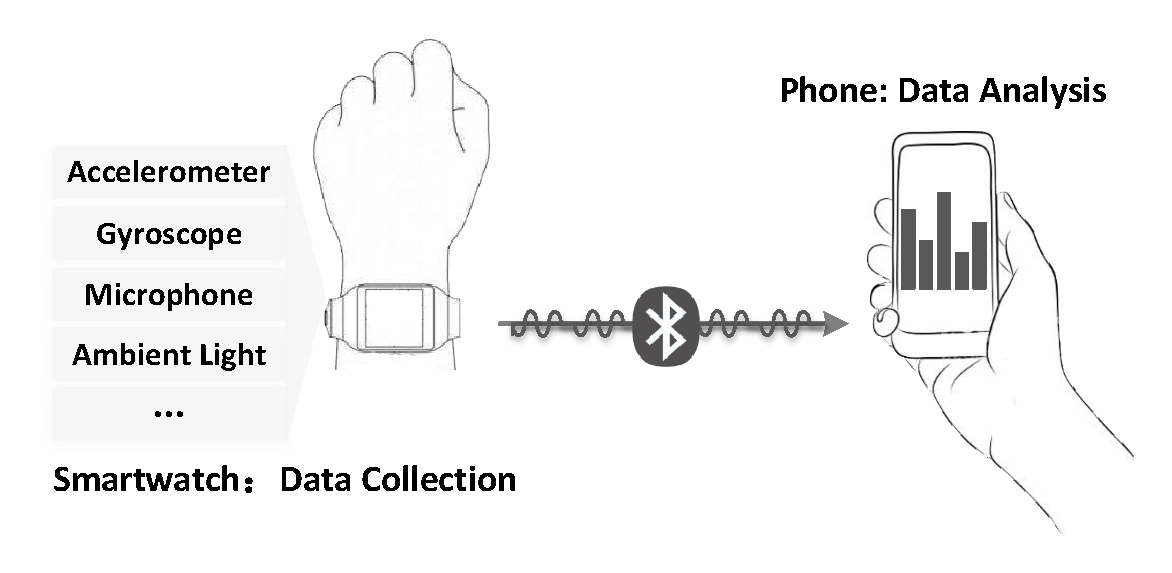
\includegraphics[width=0.5\textwidth]{Figures/datacollect.pdf}
%  \caption{Our approach detects a wide range of sleep-related activities and events using a smartwatch.}\label{fig:datacollect}
%\end{figure}

%advantages of using a smartwatch are that many users are willing to wear the device throughout the night, thus the device can remain
%relatively close to the user over the duration of sleep.



The present paper contributes by presenting the design and development of \systemname, a \emph{holistic sleep monitoring solution} that
captures rich information about sleep events, the sleep environment, and the overall quality of sleep. \systemname is the first to solely
rely on sensor information available on off-the-shelf smartwatches for capturing a wide range of sleep-related activities (see
Table~\ref{tab:test}). The key insight in {\systemname} is that sleep quality is strongly correlated with characteristics of body
movements, health related factors that can be identified from audio information, and characteristics of the sleep
environment~\cite{shelgikar2016sleep}. By using a smartwatch, the sensors are close to the user during all stages of the night, enabling
detailed capture of not only sleep cycles, but body movements and environmental changes taking place during the sleep period. capturing
these sleeping events from sensor data, however, is non-trivial due to changes in sensor measurements caused by hand motions during sleep.
To overcome this challenge, changes in sensor orientation relative to user's body need to be tracked and opportune moments where to capture
sensor data need to be detected. To address these issues, \systemname integrates a set of new methods for analysing and capturing
sleep-related information from sensor measurements available on a smartwatch. \systemname also incorporates a model that uses the detected
events to infer the user's sleep stages and sleep quality. While some prior research has examined the use of smartwatches for sleep
monitoring~\cite{pombo2016ubisleep,shelgikar2016sleep,haescher2015anomaly,borazio2012combining}, these approaches have only been able to
gather coarse-grained information about sleep and often required additional highly-specialized devices, such as pressure mattresses or
image acquisition equipment to supplement the measurements available from the smartwatch. In this paper, we demonstrate that, for the first
time, using {\em only a smartwatch}, it is possible to capture an extensive set of sleep-related information -- many of which are not
presented in prior work. Having a more comprehensive set of sleep-related events and activities available enables users to gain a deeper
understanding of their sleep patterns and the causes of poor sleep, and to make recommendations on how to improve one's sleep quality.



%We implement our approach in a prototype system called \systemname. It gathers sleep-related activities by utilizing the commonly available
%sensors on smartwatches: the accelerometer, gyroscope, microphone and ambient light sensor, etc. It then uses the tracked information to
%infer the user's sleep posture and habits -- thing like changes of body and hand positions, as well as sound events due to e.g. snoring or
%coughing.  Collecting these data can help a user to gain a deep understanding of his/her sleeping pattern and quality, and to find ways to
%improve sleep. \FIXME{ZW: The introduction is too wordy. It needs to get to the point quicker. I will get back to this later.}

  % \FIXME{ZW: This one needs to be merged with the previous paragraph.}

We evaluate \systemname through rigorous and extensive benchmark experiments conducted on data collected from fifteen participants during a
two week monitoring period. The results of our experiments demonstrate that \systemname can accurately characterize body motions and
movements during sleep, as well as capture different acoustic events. Specifically, the lowest accuracy for \systemname in our experiments
is 87\%, with the best event detection accuracy reaching up to 98\%. We also demonstrate
that \systemname can accurately detect various sleep stages and help users to better understand their sleep quality. During our experiments, six of the $15$ participants suffered from some sleep problems ($4$ with bad and $2$ with general sleep quality), all of whom were correctly identified by \systemname. Moreover, we also demonstrate that \systemname is able to correctly identify the root cause of sleep problems for the $4$ participants with bad sleep quality, whether it is due to suboptimal hand position, body posture or sleeping environment. Compared to state-of-the-art sleep monitoring systems, such as Fitbit and Sleep Hunter, the main advantage of \systemname is that can report a wider range of sleep events and provide a better understanding for the causes of sleep problems. %We show that \systemname successfully helps some of our testing users in
%finding the cause of poor sleep, 


\subsection*{Contributions}
This paper makes the following contributions:

\begin{itemize}[noitemsep]
	\item We present the design and development of \systemname (Section ~\ref{Sec:3design}), the first holistic sleep monitoring system to rely solely on sensors
available in an off-the-shelf smartwatch to capture a wide range of sleep information that characterizes overall sleep quality, user
behaviours during sleep, and the sleep environment.
	
\item We develop novel and lightweight algorithms for capturing sleep-related information on smartwatches taking into consideration
    changes in orientation and location of the device during different parts of the night. We show how to overcome specific challenges to
    effectively track events like sleep postures (Section~\ref{sec:sleeppdet}), hand positions (Section~\ref{sec:handpr}), body
    rollovers(Section~\ref{sec:bodyrollover}), micro body movement(Section~\ref{sec:microbo}), and acoustical (Section~\ref{sec:acoustic}) and
    lighting conditions (Section~\ref{sec:illumination}).


     %\textcolor{blue}{When we design these
%    algorithms, firstly, we found a key basis for sleeping posture detection that arms have common and (reasonably) stable positions in
%    each posture. Thus, we can build a mapping between the user's arms position and sleeping postures and identify the user's posture by
%    identifying periods where the hand is in a position that correlates with a specific posture. Secondly, we try to detect the position
%    of the hand based on another intuition??that is any change in hand position results in a movement trajectory that is uniquely
%    determined by the start and end position of the hand. However, we find that in practical applications, it is difficult for us to
%    obtain the starting position of the hand every time, so rely on the trajectory of the hand movement does not work. In the end, we
%    based on a key intuition is that respiratory lead to the movement of the abdomen and chest, making the acceleration signals to
%    exhibit a distinctly periodic fluctuation. We can use the occurrence of respiratory events to determine if the hand is indeed on the
%    body (abdomen or chest). Thirdly, when we detect the body rollover events, we avoided using the methods of detecting the direction of
%    rotation of the arm or the tilt of the wrist during movement of the body. Although these two methods seem to be effective, but in the
%    actual sleep process, the error they get is very large. To deal with this challenge, we incorporate the body postures to improve the
%    detection accuracy. It is based on the simple fact that the body postures are different before and after the rollover. Nextly, we
%    detect the micro body movement based on the signal duration time and the first-order derivative of the acceleration, in order to
%    realize the classification of more micro motions. In addition, we also designed two interesting algorithms, namely the detection of
%    acoustic events, changing the traditional complex algorithm multi-dimensional signal feature extraction, instead, it is through
%    mining the essential characteristics of events, that is exploiting the inherent characteristics of different acoustic event to
%    detect. And the other algorithm is illumination conditions detection, we use the movement of the hand to avoid the problem of
%    unstable reading of the light sensor.}
	

    \item We extensively evaluate the performance of \systemname using measurements collected from two-week monitoring of $15$
        participants (Section~\ref{sec:expsetup}). Our results demonstrate that \systemname can accurately capture a wide range of sleep
        events, estimate different sleep stages, and produce meaningful information about overall sleep quality
        (Section~\ref{sec:4experiment}).  We show that \systemname successfully reveals the causes of poor sleeps for some of our testing
        users and subsequently helps them improve their sleep by changing their sleep behaviours and sleeping environment
        (Section~\ref{sec:user_survey}).
\end{itemize}

%To summarize, the main contribution of this paper is the first smartwatch-based system that can capture a wider range of sleep events with a high
%accuracy. We show that, compared with existing mobile-based sleep monitoring solutions, the rich set of fine-grained sleep events given by
%o%
%ur approach can better capture a user's sleep patterns and quality across sleep stages.
